% LM_C4-134-152 (scans 134-152), second pass: checked line by line against the scans; changes in LM_C4-134-152_changes.md
\scanpage{134}

\margin{\figure{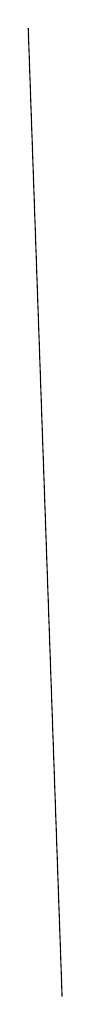
\begin{tikzpicture}\draw (0,0) -- (0.43,-12.3);\end{tikzpicture}}}

of $\mathcal M$ satisfying the following conditions

\par a) $M\longrightarrow\widetilde{\widetilde{\mathcal M}}$ (\unsure{composite} $M\longrightarrow\widetilde{\mathcal M}\longrightarrow\widetilde{\widetilde{\mathcal M}}$) is injective,

\par \deleted{b) $\unsure{\Gamma'}\ \widetilde{\widetilde{\mathcal M}}/\unsure{M|\Gamma}$}

\par hence extension

\par $(293)$\quad
\diagram{\begin{tikzcd}[ampersand replacement=\&,column sep=small]
1\arrow[r,dash]\&M\arrow[r,dash]\&\widetilde{\widetilde{\mathcal M}}\arrow[r,dash]\&\deleted{\unsure{\widetilde{\widetilde{\mathcal M}}/M}}\,\underset{\inserted{\overset{\mathrm{dfn}}{=}\widetilde{\widetilde{\mathcal M}}/M}}{\Gamma'}\arrow[r,dash]\&1
\end{tikzcd}}

\par b) \deleted{$\unsure{\widetilde{\widetilde{\mathcal M}}/M}$} $\Gamma'\overset{\mathrm{dfn}}{=}\widetilde{\widetilde{\mathcal M}}/M$ operates \uline{\unsure{faithfully}} on $M$,

\par i.e. we have
\[
\Gamma'\simeq\widetilde\Gamma=\operatorname{Im}(\Gamma\longrightarrow\operatorname{Aut}(M)).
\]

\par c) The extension $\widetilde{\widetilde{\mathcal M}}$ of $\Gamma'\simeq\widetilde\Gamma$ by $M$ is trivial (i.e. its class in $H^2(\widetilde\Gamma,M)$ is zero).

\par For such a quotient $\widetilde{\widetilde{\mathcal M}}$\inserted{ of $\widetilde{\mathcal M}$}, we recover $E$ as the set of all the splittings of the extension $\widetilde{\widetilde{\mathcal M}}$ of $\widetilde\Gamma$ by $M$, \deleted{\unsure{by|which}} on which we have $\widetilde{\mathcal M}$ operate via $\widetilde{\widetilde{\mathcal M}}$ by conjugation -- the restriction of this operation to $M\subset\widetilde{\mathcal M}$ makes $E$ an $E$-torsor (by hypothesis $(292)$).


Let us return again to the particular case that interests us. In the preceding number\textsuperscript{o} $(12^{\mathrm o})$ we verified the \deleted{\unsure{tr}} relations $(292)$, showing at the same time that this famous extension $G_{\rho,\widetilde\sigma}$ of $\widetilde\Gamma\simeq\unsure{\widehat{\mathbb Z}^{*}}\times\mathfrak S_3$ by $M^{\wedge}$ (denoted $M$ in the general considerations)

\margin{133}

% Archive printed footer (not manuscript):
% 133
% https://grothendieck.umontpellier.fr
% Université de Montpellier, UMR CNRS 5149, Case courrier 051, Place Eugène Bataillon
% 34095 Montpellier cedex 5 - France

\scanpage{135}
\mspage{715}

was trivial, and that two splittings were conjugate by an element of $M$ and only one (it is this second assertion of existence and uniqueness of conjugation that is the geometric content of $(292)$).
Moreover, we have \deleted{\unsure{thus}} indeed constructed, in number\textsuperscript{o} $11$, a surjective homomorphism
\diagram{\begin{tikzcd}[ampersand replacement=\&]
\mathcal M=\mathcal M_{0,3}\arrow[r]\&G_{\rho,\widetilde\sigma}
\end{tikzcd}}
thus making $G_{\rho,\widetilde\sigma}$ a quotient of $\mathcal M$ and even of $\widetilde{\mathcal M}$, which has the properties a) b) c) of the preceding corollary. \uline{This therefore defines for us, up to unique isomorphism, an object of the category of} $\mathcal X'$,
\deleted{i.e. a pro-covering of}
\uline{or what amounts to the same, a pro-étale covering of} $(U_{0,3\,\mathbb Q},\mathfrak S_3)\unsure{\simeq}M'_{1,1\,\mathbb Q}$,
\uline{which after \deleted{extension}\inserted{forgetting} \unsure{the operations} of} $\mathfrak S_3$ \uline{and extension of the base from} $\mathbb Q$ \uline{to} $\overline{\mathbb Q}$, \uline{becomes the universal abelian covering of} $U_{0,3\,\overline{\mathbb Q}}$.

But on the other hand the tower of Fermat coverings provides us with quite exactly such an object -- and if

\margin{134}

% Archive printed footer (not manuscript):
% 134
% https://grothendieck.umontpellier.fr
% Université de Montpellier, UMR CNRS 5149, Case courrier 051, Place Eugène Bataillon
% 34095 Montpellier cedex 5 - France

\scanpage{136}

I had not had this Fermat tower at my disposal, I certainly would not have suspected that \deleted{\unsure{$\widetilde{\widetilde{\mathcal M}}$ extension|even this extension}} subextension $\mathfrak S^{+\wedge}/\mu_{\mathfrak S}$\inserted{$=\widetilde{\mathfrak S}^{+\wedge}$} \deleted{of $\unsure{H}$} of $\widetilde H^+\simeq\mathfrak S_3$ by $M^{\wedge}$ was split!

\margin{\figure{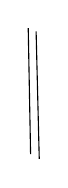
\begin{tikzpicture}\draw (0,0) -- (0.03,-1.6);\draw (0.10,-0.04) -- (0.14,-1.66);\end{tikzpicture}}}
The conjecture that presents itself at once is that these two pro-étale coverings are isomorphic -- the isomorphism between the two \unsure{is} then unique.


\deleted{\unsure{And}} This is the moment to determine the isomorphism classes of the \unsure{classes} of splittings of \inserted{the extension $\widetilde{\mathcal M}\unsure{\simeq}\mathcal M_{0,3}/[\widehat\Pi_{0,3},\widehat\Pi_{0,3}]$ of} $\Gamma=\Gamma_{\mathbb Q}\times\mathfrak S_3$ by $M^{\wedge}$, we have by the exact sequence associated with the Hochschild spectral sequence

$(294)$\quad
\diagram{\begin{tikzcd}[ampersand replacement=\&,column sep=small]
0\arrow[r,dash]\&H^1(\Gamma_{\mathbb Q},H^0(\deleted{\unsure{\widetilde\Gamma}}\mathfrak S_3,\widehat M))\arrow[r,dash]\&H^1(\unsure{\Gamma},\widehat M)\arrow[r,dash]\&H^0(\Gamma_{\mathbb Q},H^1(\mathfrak S_3,\widehat M))\arrow[d]\\
\&\&\&H^2(\Gamma_{\mathbb Q},H^0(\mathfrak S_3,M))
\end{tikzcd}}

Now we have seen that
\[
(295)\qquad H^0(\mathfrak S_3,\widehat M)=0
\qquad(\text{\unsure{and} }\overline{\mathrm m}\ H^0(\unsure{L_\rho|L_j},\unsure{\widehat M|\overline M})=0)
\]
\margin{hence $H^1(\Gamma,\widehat M)\simeq H^0(\Gamma_{\mathbb Q},H^1(\mathfrak S_3,\widehat M))$}
\deleted{\unsure{And}} Let us compute on the other hand
\[
H^1(\mathfrak S_3,\widehat M)=H^1(\mathfrak S_3,M)\otimes_{\mathbb Z}\widehat{\mathbb Z},
\]

\margin{135}

% Archive printed footer (not manuscript):
% 135
% https://grothendieck.umontpellier.fr
% Université de Montpellier, UMR CNRS 5149, Case courrier 051, Place Eugène Bataillon
% 34095 Montpellier cedex 5 - France

\scanpage{137}
\mspage{716}

which \unsure{returns} us to computing
\[
H^1(\mathfrak S_3,M)\quad ?
\]
But the study made of the extension $\mathfrak S^+/\mu_{\mathfrak S}$ of $\mathfrak S_3$ by $M$ -- which has shown us that this extension was split, and that two splittings were conjugate by a unique element of $M$, gives us in fact
\[
(296)\qquad
\left\{\begin{array}{ll}
H^0(\mathfrak S_3,M)=H^1(\mathfrak S_3,M)=0&\text{hence}\\
H^0(\mathfrak S_3,\unsure{\widehat M|\overline M})=H^1(\mathfrak S_3,\unsure{\widehat M|\overline M})=0&
\end{array}\right.
,
\]
hence finally, thanks to $(295)$, the triumphant relation
\[
(297)\qquad\boxed{H^1(\Gamma_{\mathbb Q}\times\mathfrak S_3,\widehat M)=0}\qquad !
\]

We thus find -- once again against all expectations, I confess! -- the

\uline{Theorem}\quad There exists a pro-étale \deleted{pro}covering
\margin{\figure{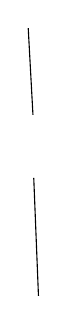
\begin{tikzpicture}\draw (0,0) -- (0.06,-1.1);\draw (0.07,-1.9) -- (0.13,-3.4);\end{tikzpicture}}}
\deleted{$\unsure{X|Z}$} $U_\infty$ of $(U_{0,3\,\mathbb Q},\mathfrak S_3)$\inserted{$=M'_{1,1\,\mathbb Q}$}, having the following property: The inverse image \inserted{$\overline U_\infty$} of $U_\infty$ over $U_{0,3\,\overline{\mathbb Q}}$ (\deleted{\unsure{without}}\inserted{\unsure{forgetting}} operations of $\mathfrak S_3$) is ``the'' universal abelian covering of $U_{0,3\,\overline{\mathbb Q}}$. For two such cover-

\margin{136}

% Archive printed footer (not manuscript):
% 136
% https://grothendieck.umontpellier.fr
% Université de Montpellier, UMR CNRS 5149, Case courrier 051, Place Eugène Bataillon
% 34095 Montpellier cedex 5 - France

\scanpage{138}

ings pro-étale over $(U_{0,3\,\mathbb Q},\mathfrak S_3)=M'_{1,1\,\mathbb Q}$, there exists a unique isomorphism from one onto the other.

We have obtained existence in \uline{two} ways: by the Fermat tower, and by the general theory of \S\,$49$ \uline{III}, applied to the present case -- which gives us a $U_\infty$ and a $U'_\infty$, each described up to unique isomorphism! The uniqueness theorem follows from the preceding little calculation -- I was afraid of the ``big'' \deleted{$\unsure{H^1(\Gamma_{\mathbb Q},\widehat M)\simeq H^1(\Gamma}$}
\[
H^1(\Gamma_{\mathbb Q},\widehat M)\simeq
M\otimes_{\mathbb Z}\underbrace{H^1(\Gamma_{\mathbb Q},T_{\unsure{\infty|*}}(G_m))}_{\widehat{\mathbb Q^{*}}},
\]
but in the end it is the vanishing of $H^{i}(\mathfrak S_3,M)$ for $i=0,1$ that implies (without knowing anything about $\Gamma_{\mathbb Q}$!) that of $H^1(\Gamma_{\mathbb Q}\times\mathfrak S_3,\widehat M)$, which ensures the uniqueness we needed.

\margin{137}

% Archive printed footer (not manuscript):
% 137
% https://grothendieck.umontpellier.fr
% Université de Montpellier, UMR CNRS 5149, Case courrier 051, Place Eugène Bataillon
% 34095 Montpellier cedex 5 - France

\scanpage{139}
\mspage{717}

\deleted{For} The preceding theorem completely elucidates, it seems to me, the arithmetico-geometric meaning (in terms of the Fermat tower) of the homomorphism ((218) page~695')
\[
\mathcal M=N_{1,1}^{\text{ét}}\longrightarrow G_{\rho,\sigma}\simeq\widehat{\mathbb Z}^{*}\mathbin{.}\mathfrak S_{\unsure{\bullet|0}}^{+\wedge}
\]
obtained in section 11°) by purely algebraic means --- or at least that of the slightly weaker homomorphism
\[
\mathcal M\longrightarrow\overbrace{G_{\rho,\sigma}/\mu_{\mathfrak S}}^{\inserted{G_{\rho,\widetilde{\sigma}}\overset{\mathrm{dfn}}{=}}}\simeq\widehat{\mathbb Z}^{*}\mathbin{.}\mathfrak S^{+\wedge}/\mu_{\mathfrak S}
\]
which factors \deleted{through} into a homomorphism
\[
\underbrace{\widetilde{\mathcal M}}_{\inserted{\text{denoted }\mathcal M\text{ in the preceding pages}}}\overset{\mathrm{dfn}}{=}\mathcal M/(\mu_{\mathcal M}=\mu_{\mathfrak S_{\unsure{0|\bullet}}})\longrightarrow G_{\rho,\widetilde{\sigma}}
\qquad\text{extension of }\widetilde\Gamma=\widehat{\mathbb Z}^{*}\times\mathfrak S_3\text{ by }M^\wedge.
\]

The passage from $G_{\rho,\sigma}^{\deleted{\unsure{\sim}}}$ to $G_{\rho,\widetilde{\sigma}}$, from the present point of view, had as its essential role (a posteriori!) to provide an extension by $M^\wedge$ (playing the role of an identity component) of a group operating \uline{faithfully} on $M^\wedge$, which was not the case for the extension $G_{\rho,\sigma}$ of $\widehat{\mathbb Z}^{*}\times H^+$ by $M^\wedge$, since the \deleted{\unsure{center|element}} \inserted{center $\mu_{H^+}=\{1,\unsure{\omega_{H^+}}\}$ \deleted{\unsure{$H^+$}} of $H^+$} operated trivially.
\margin{138}

% Archive printed footer (not manuscript):
% 138
% https://grothendieck.umontpellier.fr
% Université de Montpellier, UMR CNRS 5149, Case courrier 051, Place Eugène Bataillon
% 34095 Montpellier cedex 5 - France